\documentclass[11pt]{article}
\usepackage[a4paper,margin=2.6cm]{geometry}
\usepackage[T1]{fontenc}
\usepackage[utf8]{inputenc}
\usepackage{lmodern}
\usepackage{amsmath,amssymb,amsthm,mathtools}
\usepackage{booktabs,multirow,array}
\usepackage{graphicx}
\usepackage[font=small,labelfont=bf]{caption}
\usepackage{subcaption}
\usepackage[numbers,sort&compress]{natbib}
\usepackage{xcolor}
\usepackage[colorlinks=true,linkcolor=blue!50!black,citecolor=blue!50!black,urlcolor=blue!50!black]{hyperref}
\usepackage{microtype}
\usepackage{enumitem}
\usepackage[section]{placeins}

\newtheorem{proposition}{Proposition}
\newtheorem{lemma}[proposition]{Lemma}
\newtheorem{corollary}[proposition]{Corollary}
\theoremstyle{definition}
\newtheorem{definition}{Definition}
\newtheorem{remark}{Remark}
\newtheorem{observation}{Observation}

\newcommand{\R}{\mathbb{R}}
\newcommand{\rms}{\operatorname{rms}}
\newcommand{\diag}{\operatorname{diag}}
\newcommand{\E}{\mathbb{E}}
\newcommand{\zH}{z_H}
\newcommand{\zL}{z_L}
\newcommand{\Bk}{\mathcal{B}}
\makeatletter\newcommand{\tabinput}[1]{\@@input #1 }\makeatother

\title{Damped two-stream couplings in equilibrium reasoners:\\
attractor geometry, inner loops and test-time scaling on Sudoku-Extreme}
\author{H\aa kon Noren}
\date{Working note, \today}

\begin{document}
\maketitle

\begin{abstract}
Equilibrium Reasoners (EqR) iterate one shared block on two latent states and reach high accuracy on
Sudoku-Extreme by spending test-time compute: more iterations (depth), more random starts (breadth), and
Langevin noise. We replace EqR's self-reading update by two-stream \emph{kick} and \emph{relax} couplings in which
each stream is driven only by the other, so that every update is an invertible shear followed by a constant
scaling, and we study which properties of the resulting maps decide accuracy, depth scaling, breadth and the effect of noise.
On the theory side we show that (i) the force block has unit per-token RMS, so the state at a fixed point is
an exact, rate-determined multiple of a unit vector, which fixes the scale against which test noise acts;
(ii) the volume constraint of the coupled maps is not binding for any trained model except one with near-identity rates;
(iii) symmetric relaxation without common-mode damping has an exactly neutral mode, and damping it is what makes relax work;
(iv) alternating couplings have no implicit inner fixed-point problem, while EqR's inner loop does; and
(v) a relaxed self-map with strong negative feedback undergoes a period-doubling (flip) bifurcation, which a
two-copy (``twin'') coupling turns back into a fixed point.
Numerically, on 14 checkpoints we measure Jacobian spectra, path independence, selection, and escape under noise.
Right answers are attracting fixed points and wrong end states are not, in every working model, so convergence-based
selection is nearly perfect and accuracy is limited by \emph{coverage}. Test noise helps by selectively
destabilising wrong attractors below an arm-specific breakdown level. EqR differs from the coupled maps in being near
critical at its answers ($\rho\approx 0.93$--$0.97$ per outer iteration against $0.53$--$0.73$), in being more path
independent, and in an inner loop that, with training, goes through a flip bifurcation into an exact 2-cycle.
With training to 50k steps, EqR pulls ahead of the coupled maps on every metric.
All results are single-seed.
\end{abstract}

\tableofcontents

%=====================================================================================================
\section{Introduction}

Looped (weight-tied, recurrent-depth) reasoners solve constraint problems such as Sudoku by iterating one block
many times \cite{wang2025hrm,jolicoeur2025trm,huang2026eqr,geiping2025recurrent}. Equilibrium Reasoners
(EqR, \cite{huang2026eqr}) add three ingredients to TRM-style recursion: random initial states, Langevin noise
in the state, and an explicit view of reasoning as convergence to an attractor. At test time EqR scales
\emph{depth} (iterations), \emph{breadth} (random starts per puzzle, with an answer chosen by convergence) and noise.

This note asks which properties of the iteration map make these work. We keep EqR's data, block, training recipe
and evaluator, and replace only the state update by two-stream couplings in the spirit of conformal symplectic
integrators \cite{mclachlan2001conformal,franca2020conformal} and momentum networks \cite{sander2021momentum}:
\begin{align*}
\textbf{kick:}&\quad L \leftarrow a\,\bigl(L + \Bk(H+x)\bigr), && H \leftarrow bH + \Bk(L+x),\\
\textbf{relax:}&\quad L \leftarrow aL + (1-a)\bigl(cH + \Bk(H+x)\bigr), && H \leftarrow bH + (1-b)\bigl(cL + \Bk(L+x)\bigr),
\end{align*}
with $a=e^{-\gamma}$, $b=e^{-\alpha}$, $c=e^{-\delta}$. Each stream is driven only by the other stream, so every
update is invertible with a state-independent Jacobian determinant. We then compare these maps with EqR in
accuracy (\S\ref{sec:acc}), test-time scaling (\S\ref{sec:tts}) and a direct dynamical analysis of trained
checkpoints (\S\ref{sec:maps}), guided by a small amount of theory (\S\ref{sec:theory}).

\paragraph{Summary of findings.}
\begin{enumerate}[leftmargin=*,itemsep=1pt]
\item \textbf{Certification is easy; coverage is hard.} In every working model right answers are attracting fixed points
($\rho<1$) and wrong end states are not ($\rho>1$). Convergence, the halting head and a Sudoku validity check therefore pick
the right start almost whenever one exists (AUROC $\approx 1$); what separates models is how often random starts land in the
right basin (\S\ref{sec:select}).
\item \textbf{Noise acts on wrong attractors first.} Under noise $\sigma$ below an arm-specific breakdown level $\sigma^\star$ right
answers are never lost, while $15$--$33\%$ of wrong end states are rescued (\S\ref{sec:escape}), as in Hopfield
networks at finite temperature \cite{amit1985storing,coolen2000statics}. $\sigma^\star$ depends on the state scale, which is fixed
exactly by the rates (Prop.~\ref{prop:scale}), and on how strongly the answers attract.
\item \textbf{EqR is near critical and more path independent.} EqR's right answers have $\rho\approx0.87\to0.93\to0.97$
(20k, 50k, released) per outer iteration, matching the $0.89$--$0.97$ reported for converged Sudoku loopers
\cite{labovich2026stability}; the coupled maps contract much harder ($0.53$--$0.73$). EqR's random starts reach fewer distinct
answers (1.6 per puzzle at 50k against 2.6 for relax and 3.2 for kick).
\item \textbf{EqR's inner loop flips.} With $\zH$ frozen, EqR's inner map has a stable fixed point at 20k steps but sits on an exact
2-cycle at 50k (Prop.~\ref{prop:flip}); its leading Jacobian eigenvalue moves from $\approx\pm0.6$ to $\approx-1$ and, in the released
checkpoint, to $\approx-2$. The cycle is invisible to the readout: odd inner-loop lengths work as well as even ones.
\item \textbf{Damping matters, volume does not.} The volume bound of the coupled maps (Prop.~\ref{prop:volume}) is irrelevant for all
trained models except a near-identity kick; relax without common-mode damping has an exactly neutral mode (Prop.~\ref{prop:neutral})
and fails, and accuracy improves monotonically as the merged-state retention falls from $1$ to $\approx0.2$ (\S\ref{sec:acc}).
\item \textbf{Training length favours EqR.} At 20k steps relax ties EqR with enough test-time compute; at 50k EqR leads on every metric
(depth 1024: $97.1$ vs.\ $92.5$; depth 64 with 128 starts: $98.7$ vs.\ $96.6$).
\end{enumerate}

%=====================================================================================================
\section{Setting}\label{sec:setting}

\subsection{EqR}
A puzzle is embedded as $x\in\R^{n\times d}$ ($n=97$ positions: 16 puzzle-embedding slots and 81 cells; $d=512$). The
shared block $\Bk:\R^{n\times d}\to\R^{n\times d}$ is two post-norm layers, each $v\mapsto N(v+\mathrm{MLP}_t(v))$ followed by
$v\mapsto N(v+\mathrm{SwiGLU}(v))$, where $\mathrm{MLP}_t$ mixes tokens and $N$ is RMS normalisation \emph{without gain},
$N(y)_i = y_i/\rms(y_i)$ row-wise.

\begin{definition}[EqR update {\cite{huang2026eqr}}]
With $\lambda=0.95$ and noise $\xi\sim\mathcal N(0,\sigma^2 I)$ drawn afresh after every update, one \emph{latent recursion} is
\[
\zL \leftarrow (1-\lambda)\zL + \lambda\,\Bk(\zL+\zH+x) + \xi\quad(\text{6 times}),\qquad
\zH \leftarrow (1-\lambda)\zH + \lambda\,\Bk(\zH+\zL) + \xi .
\]
One \emph{outer iteration} (one ACT step) is three recursions, i.e.\ 21 block evaluations; the readout decodes $\zH$.
Training differentiates only the last recursion (7 evaluations), carries the state across outer iterations detached,
starts from random states (truncated normal, std 1), and uses $\sigma=0.01$.
\end{definition}

\subsection{Coupled updates}
\begin{definition}[Kick and relax]\label{def:coupled}
Let $a=e^{-\gamma},\ b=e^{-\alpha},\ c=e^{-\delta}\in(0,1]$. A \emph{half-step} updates one stream from the other:
\begin{align*}
\text{kick:}&\quad L\leftarrow a\,(L+\Bk(H+x)), && H\leftarrow bH+\Bk(L+x),\\
\text{relax:}&\quad L\leftarrow aL+(1-a)\bigl(cH+\Bk(H+x)\bigr), && H\leftarrow bH+(1-b)\bigl(cL+\Bk(L+x)\bigr).
\end{align*}
A recursion is the alternating sequence $H,L,H,L,H,L,H$ (7 evaluations); three recursions form an outer iteration (21 evaluations,
7 differentiated), exactly as in EqR. The readout decodes $N(H)$. Noise is added after every half-step.
\end{definition}

\noindent Variants (Table~\ref{tab:arms}): \emph{$x\to L$ only} drops $x$ from $H$'s force (EqR's choice); \emph{self-read} adds the updated
stream to its own force input ($L\leftarrow\dots\Bk(L+H+x)$), which breaks invertibility; \emph{inner loop} uses EqR's order
($L^6H$) with self-read; \emph{twin} doubles $L$ into $L,L'$ that read each other (\S\ref{sec:twin}).

\begin{table}[t]
\centering\small
\caption{Arms. Rates are fixed unless stated. ``Positive'' kick learns $\gamma=0.05+\mathrm{softplus}(\cdot)$ from $\gamma=1$.
Invertible: every update is a shear followed by a constant scaling.}\label{tab:arms}
\begin{tabular}{@{}p{3.7cm}p{4.1cm}p{3.3cm}cc@{}}
\toprule
arm & update & rates & invertible & round \\
\midrule
EqR & self-read, order $L^6H$ & $1-\lambda=0.05$ & no & ref. \\
kick: fixed, learned, positive & kick & $\gamma{=}\alpha{=}0.005$; learned; learned $\ge0.05$ & yes & 1 \\
relax, $\delta\in\{0,\tfrac14,1\}$ & relax & $\gamma=\alpha=3$ & yes & 1 \\
relax / kick, $x\to L$ only & no $x$ in $H$'s force & as above & yes & 2 \\
relax $\delta{=}1$, $x\to L$, self-read & forces read own stream & $\gamma=\alpha=3$ & no & 2 \\
relax, $\delta\in\{2,3\}$ & relax & $\gamma=\alpha=3$ & yes & 3 \\
twin $L$, $\delta\in\{1,2\}$ & $L,L'$ read each other, order $LL'LL'LL'H$ & $\gamma=\alpha=3$ & yes$^\ast$ & 3 \\
inner loop, self-read & self-read relax, order $L^6H$ & $\gamma=\alpha=3$, $\delta=1$ & no & 3 \\
\bottomrule
\end{tabular}\\[2pt]
{\footnotesize $^\ast$Every update reads only streams it does not change; no inverse is implemented.}
\end{table}

\subsection{Evaluation}
\emph{Depth} $D$ is the number of outer iterations; \emph{breadth} $B$ is the number of random starts per puzzle. For $B>1$ an answer
is chosen by: the most converged start (EqR's score, the logit change over the last three iterations; ``converged''); the mean
accuracy of the four most converged (``top-4'', EqR's headline); plurality of full grids (``vote''); the largest halting logit;
or a label-free \emph{Sudoku verifier} (a grid with no rule violations that keeps the givens; Sudoku-Extreme puzzles have unique
solutions, so this equals ``some start is right'', ``any''). Test noise defaults to $\sigma=0.5$ as in EqR's released
evaluation. Sample sizes: whole test set (423k) for in-training accuracy at 16 iterations, the first 2048 puzzles for
depth$\times$breadth, and the first 256 puzzles $\times16$ starts $\times256$ iterations for the dynamical analysis.

%=====================================================================================================
\section{Theory}\label{sec:theory}

\subsection{State scale}

\begin{lemma}[Unit-RMS force]\label{lem:unit}
Every token row of $\Bk(u)$ has RMS exactly one (up to the normalisation $\epsilon$).
\end{lemma}
\begin{proof}$\Bk$ ends with $N$, which divides each row by its RMS and has no gain parameter.\end{proof}

\begin{proposition}[Fixed-point scale]\label{prop:scale}
At a noise-free fixed point, with $f$ the (unit-RMS) force evaluated there:
\begin{enumerate}[label=(\alph*),itemsep=0pt]
\item EqR: $\zL^\ast = \Bk(\cdot)$, so $\rms(\zL^\ast)=1$, and likewise $\zH^\ast$;
\item kick: $L^\ast=\tfrac{a}{1-a}f_L$ and $H^\ast=\tfrac{1}{1-b}f_H$, so $\rms(L^\ast)=\tfrac{a}{1-a}$, $\rms(H^\ast)=\tfrac{1}{1-b}$;
\item relax with merged streams $H^\ast=L^\ast=z^\ast$: $z^\ast=\tfrac{1}{1-c}\,\Bk(z^\ast+x)$, so $\rms(z^\ast)=\tfrac{1}{1-c}$; for $c=1$ there is no fixed point unless $\Bk(z^\ast+x)=0$.
\end{enumerate}
\end{proposition}
\begin{proof}Set new state equal to old state in each update and solve; e.g.\ for kick $L^\ast=a(L^\ast+f_L)$ gives $L^\ast=\frac{a}{1-a}f_L$; for merged relax
$z^\ast=az^\ast+(1-a)(cz^\ast+f)$ gives $(1-a)(1-c)z^\ast=(1-a)f$. Lemma~\ref{lem:unit} gives the RMS.\end{proof}

\noindent The identity is exact per token. The measured endpoint RMS matches it to within $1\%$ for every EqR, kick and merged-relax
checkpoint (Figure~\ref{fig:scale}, Table~\ref{tab:rates}; it does not apply to the unmerged $x\to L$ relax arms or to $\delta=0$, which has no fixed point): e.g.\ kick (positive, 20k) $L$: predicted $0.64$, measured $0.64$; merged relax $\delta=1$:
$1.58$ vs.\ $1.58$; relax $\delta=\frac14$: $4.52$ vs.\ $4.51$; kick (fixed): $200$ vs.\ $199.8$.

\begin{corollary}[Relative noise]
Isotropic noise $\sigma$ acts on a stream of scale $s$ as relative noise $\sigma/s$. At $\sigma=0.5$ this is $0.5$ for EqR, $\approx0.3$ for
merged relax ($\delta=1$), and $\approx0.8$ for the $L$ stream of positive kick at 20k (whose $L$ grows to $0.81$ by 50k as $\gamma$ falls).
\end{corollary}

\subsection{Volume}

\begin{proposition}[Volume bound]\label{prop:volume}
Each coupled half-step is a shear $(s,o)\mapsto(s+g(o),o)$ composed with a constant diagonal scaling, so for one outer
iteration with $n_L$ $L$-half-steps and $n_H$ $H$-half-steps (per channel and token)
$\ \log|\det J| = -nd\,(n_L\gamma+n_H\alpha)$. Hence the geometric mean of $|\mu|$ over the $2nd$ eigenvalues of $J$ is
$e^{-(n_L\gamma+n_H\alpha)/2}$, and in particular $\rho(J)\ge e^{-(n_L\gamma+n_H\alpha)/2}$ at every fixed point.
\end{proposition}
\begin{proof}A shear has unit Jacobian determinant; the scaling contributes $a^{nd}$ or $b^{nd}$ per half-step (for relax the
cross term $(1-a)cH$ is part of the shear). Multiply over the 21 half-steps. The spectral radius is at least the geometric mean
of the moduli.\end{proof}

\begin{remark}The shears are symplectic only if $\partial g/\partial o$ is symmetric, which a learned block is not, so the maps are
volume-contracting at a constant rate but not conformal symplectic: there is no eigenvalue pairing $\mu\leftrightarrow e^{-\cdot}/\mu$
\cite{mclachlan2001conformal}, only the determinant constraint.\end{remark}

\noindent The bound is $2\times10^{-14}$ per outer iteration for relax (rate 3), $9\times10^{-6}$ and $7\times10^{-7}$ for positive kick
(20k, 50k), $0.017$ for learned kick, but $0.949$ for fixed kick ($\gamma=\alpha=0.005$). Only the last is constrained: it cannot contract,
and indeed its end states have $\rho=1.01$ and it keeps a right answer only $42\%$ of the time even at $\sigma=0.1$ (Table~\ref{tab:escape}).

\subsection{The neutral mode of undamped relaxation}

\begin{proposition}[Common mode]\label{prop:neutral}
With the forces frozen, the linear part of the relax half-steps acting on $(L,H)$ per channel is
$M_L=\begin{psmallmatrix}a&(1-a)c\\0&1\end{psmallmatrix}$, $M_H=\begin{psmallmatrix}1&0\\(1-b)c&b\end{psmallmatrix}$.
For $c=1$ both are row-stochastic, so $(1,1)^\top$ is a fixed vector of every product: the common mode is exactly neutral ($\mu=1$).
For $c<1$ the row sums are $a+(1-a)c<1$ and $b+(1-b)c<1$, so every product has spectral radius below one.
With $a=b$ and merged streams the common mode is retained at the rate $r=a+(1-a)c$ per half-step.
\end{proposition}
\begin{proof}Row-stochastic matrices have eigenvalue $1$ with eigenvector $\mathbf 1$; a nonnegative matrix's spectral radius is
at most its maximum row sum.\end{proof}

\noindent Relax with $\delta=0$ therefore drifts along the force (endpoint RMS $\approx4\times10^3$, $\rho=1.00$ at its end states)
and reaches only $13\%$. Accuracy rises as the retention $r$ falls (Figure~\ref{fig:retention}); EqR's own self-retention is $1-\lambda=0.05$.

\subsection{Inner fixed-point problems}\label{sec:twin}

\begin{proposition}[Alternating couplings have an explicit inner equilibrium]\label{prop:explicit}
With $H$ frozen, repeated $L$ half-steps converge geometrically at rate $a$ to
$\Lambda(H)=cH+\Bk(H+x)$ (relax) or $\Lambda(H)=\tfrac{a}{1-a}\Bk(H+x)$ (kick), each a single block evaluation.
In EqR the inner equilibrium solves the implicit equation $\zL=\Bk(\zL+\zH+x)$, which takes iteration.
\end{proposition}
\begin{proof}The force on $L$ does not depend on $L$, so the $L$ update is affine in $L$ with slope $a$.\end{proof}

\noindent In the language of two-timescale iterations \cite{borkar1997twotimescale}, EqR's fast variable tracks an implicitly defined
equilibrium $\Lambda(\zH)$ between slow updates, whereas in the alternating couplings $\Lambda$ is one explicit layer, so the coupled
models are effectively single-latent maps (and relax's streams merge, $\cos(H,L)=1.00$). EqR's and TRM's ablations put the cost of a
single latent at $\approx10$ points \cite{huang2026eqr,jolicoeur2025trm}. The twin coupling restores an implicit inner problem:

\begin{proposition}[Twins are a two-copy doubling]\label{prop:twin}
Let $G(z)=cz+\Bk(z+H+x)$ for frozen $H$. The twin updates
$L\leftarrow aL+(1-a)G(L')$, $L'\leftarrow aL'+(1-a)G(L)$ with $a<1$ have a fixed point $(p,q)$ if and only if $p=G(q)$ and $q=G(p)$,
i.e.\ $p$ is a fixed point of $G\circ G$. Thus the twins represent both fixed points ($p=q$) and period-2 orbits ($p\neq q$) of the
self-reading map $G$ as fixed points.
\end{proposition}
\begin{proof}At a fixed point $p=ap+(1-a)G(q)$, i.e.\ $p=G(q)$, and symmetrically $q=G(p)$.\end{proof}

\begin{remark}This is the construction used to analyse synchronous Hopfield dynamics: a synchronously updated symmetric network
converges to fixed points or 2-cycles, and its two-copy bipartite version, updated sequentially, has exactly these as fixed points
\cite{goles1981periodic,bruck1990convergence}.\end{remark}

\subsection{Flip bifurcation of relaxed self-maps}

\begin{proposition}[Period doubling]\label{prop:flip}
Let $F(z)=(1-\lambda)z+\lambda\tilde\Bk(z)$ and let $\mu$ be a real eigenvalue of $D\tilde\Bk$ at a fixed point $z^\ast$. Then
$1-\lambda+\lambda\mu$ is an eigenvalue of $DF(z^\ast)$; the direction is stable iff $1-\tfrac2\lambda<\mu<1$. As $\mu$ decreases through
$1-\tfrac2\lambda$ ($=-1.105$ at $\lambda=0.95$) the eigenvalue of $DF$ crosses $-1$, and generically a period-2 orbit is born (flip
bifurcation). Smaller step sizes $\lambda<2/(1-\mu)$ restore stability.
\end{proposition}
\begin{proof}$DF=(1-\lambda)I+\lambda D\tilde\Bk$ shares eigenvectors with $D\tilde\Bk$. The flip-bifurcation statement is the standard
normal-form result for a simple eigenvalue crossing $-1$.\end{proof}

\noindent Strong negative feedback ($\mu<-1$) is natural for Sudoku, whose constraints are mutual exclusions. The stability region
and the measured values for EqR are drawn in Figure~\ref{fig:flip}; damping of this kind is also the mechanism behind the
fixed-point reasoners of \cite{movahedi2026fixedpoint}.

\subsection{Certification and noise}

EqR bounds the distance to a fixed point by the residual under local contraction ($\|z-z^\ast\|\le\|R(z)\|/(1-L)$) and turns this into a
correctness certificate when the output margin is large \cite[App.~A.1]{huang2026eqr}. The certificate needs right answers to be
contracting and wrong ones not to be; we measure exactly this in \S\ref{sec:spectra}. For noise, along a normal eigen-direction with
eigenvalue $\mu$ the linearised stationary variance is $\sigma^2/(1-|\mu|^2)$: near-critical directions amplify noise, and a basin is left
once the fluctuations reach its boundary. In Hopfield networks spurious mixture states lose stability at a lower temperature than
retrieval states \cite{amit1985storing,coolen2000statics}; noise then selects the right attractors. Section~\ref{sec:escape} tests this.

%=====================================================================================================
\section{Accuracy and training}\label{sec:acc}

\begin{table}[t]
\centering\small
\caption{Accuracy at training noise ($\sigma=0.01$), one start. Exact@16: whole test set; @64/@256: first 49{,}152 puzzles.
$O$: right at 16 but wrong at 256; $\Delta y$: prediction changed between 16 and 256.}\label{tab:main}
\setlength{\tabcolsep}{4.5pt}
\begin{tabular}{@{}llrrrrrr@{}}
\toprule
arm & steps & ex@16 & cell@16 & ex@64 & ex@256 & $O_{16\to256}$ & $\Delta y_{16\to256}$ \\
\midrule
\tabinput{tables/tab_main.tex}
\bottomrule
\end{tabular}
\end{table}

Table~\ref{tab:main} and Figure~\ref{fig:training} give the accuracies. Our EqR reproduces the paper (85.8 at 16 iterations and 92.1 at 64
after 50k steps, against 86.4 and 93.0 \cite{huang2026eqr}). At 20k steps the two best couplings, relax $\delta=1$ and positive kick, trail
EqR by about six points at 16 iterations; the gap does not close with training (7.5 points at 50k) and widens with depth (10.5 points at
256 iterations). Fixed small rates fail (Prop.~\ref{prop:volume}, \ref{prop:neutral}).

\begin{figure}[t]
\centering
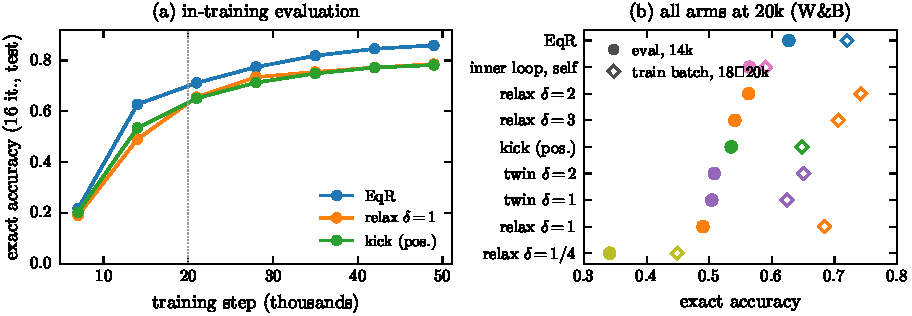
\includegraphics[width=\textwidth]{figures/fig_training.pdf}
\caption{(a) In-training evaluation (whole test set, 16 iterations) of the three arms extended to 50k steps. (b) All round-three
arms and references at 20k: evaluation at 14k (filled) and training-batch accuracy averaged over steps 18--20k (open).}\label{fig:training}
\end{figure}

\paragraph{Round two: input injection and self-reading.} Giving $x$ only to $L$ (as EqR does) costs $12$ points for relax and $7$ for kick.
For relax it separates the streams ($\cos(H,L)$ $1.00\to0.77$) but each stream is then driven only by the other. Adding self-reading
recovers $10$ of the $12$ points ($51.7\to61.7$), but only to the level of plain merged relax ($63.9$), which already reads itself in
effect (its streams coincide). Self-reading without an inner loop is therefore not what EqR has over relax.

\paragraph{Round three: damping and inner loops (20k, preliminary).} Table~\ref{tab:round3} and Figure~\ref{fig:retention}.
Lowering the merged-state retention from $0.40$ ($\delta=1$) to $0.18$ ($\delta=2$) gains seven points at 14k, and $\delta=3$ ($r=0.10$) is
slightly worse. The twins keep $H$ apart from $L$ ($\cos=0.25$--$0.45$) but are not better than relax $\delta=1$ at 14k; the inner-loop
reference is the best new arm at 14k. Whether an inner loop pays off may only show later in training, as EqR's own advantage grew
between 20k and 50k; three arms are being extended to 50k.

\begin{figure}[t]
\centering
\begin{minipage}[t]{0.49\textwidth}\centering
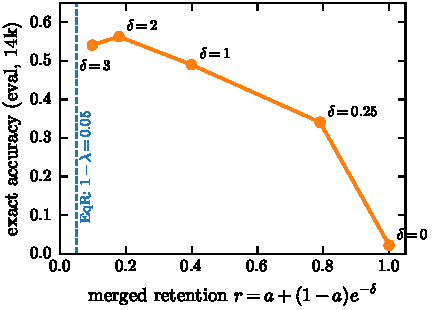
\includegraphics[width=\textwidth]{figures/fig_retention.pdf}
\caption{Relax, rate 3: accuracy at 14k against the retention $r$ of the merged state (Prop.~\ref{prop:neutral}).}\label{fig:retention}
\end{minipage}\hfill
\begin{minipage}[t]{0.49\textwidth}\centering
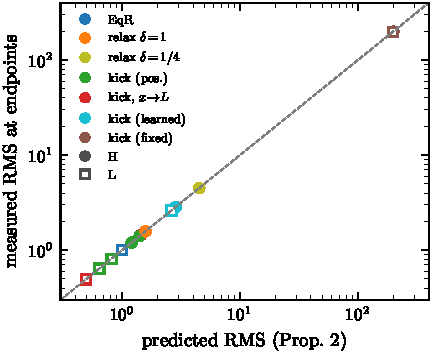
\includegraphics[width=\textwidth]{figures/fig_scale.pdf}
\caption{Endpoint state RMS against Prop.~\ref{prop:scale} ($H$ filled, $L$ open); all trained arms with a fixed point.}\label{fig:scale}
\end{minipage}
\end{figure}

\begin{table}[t]
\centering\small
\caption{Round three at 20k (W\&B). Eval: whole test set, 16 iterations, at 14k. Train: training-batch exact accuracy averaged over
18--20k (depends on halting). $\cos(H,L)$ and mean ACT steps over the same window.}\label{tab:round3}
\begin{tabular}{@{}lrrrr@{}}
\toprule
arm & eval@14k & train 18--20k & $\cos(H,L)$ & ACT steps\\
\midrule
\tabinput{tables/tab_round3.tex}
\bottomrule
\end{tabular}
\end{table}

%=====================================================================================================
\section{Test-time scaling}\label{sec:tts}

\begin{figure}[t]
\centering
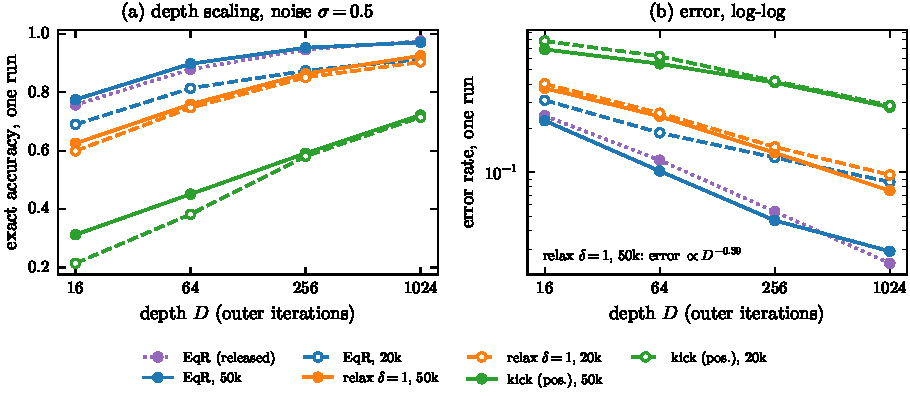
\includegraphics[width=\textwidth]{figures/fig_depth.pdf}
\caption{One-run accuracy against depth at $\sigma=0.5$ (first 2048 test puzzles). Dashed/open: 20k steps; solid/filled: 50k; dotted:
EqR's released checkpoint. (b) The error of relax falls like a power of depth; EqR's falls faster and then flattens near $3\%$.}\label{fig:depth}
\end{figure}

\begin{table}[t]
\centering\small
\caption{Test-time scaling at $\sigma=0.5$, first 2048 test puzzles. Left: one start at depth $D$. Right: depth 64 with 128 starts, by
selection rule (best in bold). The released EqR gives 98.6 top-4, as in EqR's README.}\label{tab:scaling}
\begin{tabular}{@{}llrrrr|rrrr@{}}
\toprule
& & \multicolumn{4}{c|}{one run, depth $D$} & \multicolumn{4}{c}{depth 64, 128 starts}\\
arm & steps & 16 & 64 & 256 & 1024 & converged & top-4 & vote & any \\
\midrule
\tabinput{tables/tab_scaling.tex}
\bottomrule
\end{tabular}
\end{table}

Figure~\ref{fig:depth} and Table~\ref{tab:scaling}. All working models improve steadily with depth. At 20k, relax ties EqR once compute is
large (depth 1024: $90.4$ vs.\ $91.4$; depth 64 with 128 starts, most converged: $95.9$ vs.\ $95.7$). At 50k EqR leads everywhere. Relax's
error decays like $D^{-0.39}$ without saturating, so it would need more than an order of magnitude more iterations to match EqR at 50k.

\begin{figure}[t]
\centering
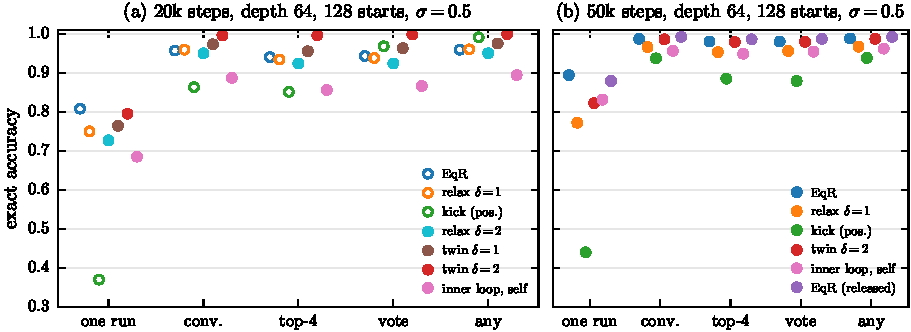
\includegraphics[width=\textwidth]{figures/fig_breadth.pdf}
\caption{Depth 64, 128 starts, $\sigma=0.5$: accuracy by selection rule. At 20k positive kick has the best vote and ``any'' but the worst
single run and convergence selection; by 50k this has reversed.}\label{fig:breadth}
\end{figure}

Positive kick at 20k is the outlier (Figure~\ref{fig:breadth}): at $\sigma=0.5$ a single run is right only $37\%$ of the time, yet some start is right
for $99.1\%$ of puzzles and a plurality vote over 128 starts reaches $96.8\%$, the best of the 20k models. Its relative noise is about $1.6$ times
EqR's (Corollary~1), which pushes it into a high-diversity regime; at noise $0.25$ its single run is $69\%$. By 50k its $L$ stream has grown (Prop.~\ref{prop:scale})
and the regime is gone (any $93.8$, vote $87.9$).

%=====================================================================================================
\section{Dynamics of the trained maps}\label{sec:maps}

All quantities in this section use the noise-free map unless stated, in float32, on the first 256 test puzzles with 16 random starts and 256
outer iterations, at the checkpoints' EMA weights.

\subsection{Selection is solved; coverage is not}\label{sec:select}

\begin{table}[t]
\centering\small
\caption{Multistart (256 puzzles, 16 starts, depth 256). ``conv.'': most converged; ``$q$'': largest halting logit; verifier: valid
Sudoku keeping the givens. AUROC of EqR's convergence score for right vs.\ wrong runs. ``answers'': mean number of distinct final grids per puzzle.}\label{tab:select}
\setlength{\tabcolsep}{4.5pt}
\begin{tabular}{@{}llrrrrrrrrr@{}}
\toprule
arm & steps & single & any & vote & conv. & $q$ & verifier & AUROC & answers & $\Delta$PI \\
\tabinput{tables/tab_select.tex}
\bottomrule
\end{tabular}
\end{table}

Table~\ref{tab:select}. For EqR and relax at $\sigma\le0.5$, the most converged start, the start with the largest halting logit and the verifier all
agree with ``any'': whenever some start is right, each rule finds it, and the convergence score separates right from wrong runs with AUROC
$0.98$--$1.00$ (Figure~\ref{fig:auroc}). The exceptions are informative: relax $\delta=\frac14$ at $\sigma=0$ (AUROC $0.53$; its right end states are not contracting,
$\rho=1.16$) and positive kick at 20k under $\sigma=0.5$ (AUROC $0.86$), the regime of its vote advantage. The differences between models are in
\emph{coverage} and in single-run accuracy, and these track path independence: at 50k EqR's starts reach $1.6$ distinct answers per puzzle,
relax's $2.6$ and kick's $3.2$ (Figure~\ref{fig:noise}c).

\begin{figure}[t]
\centering
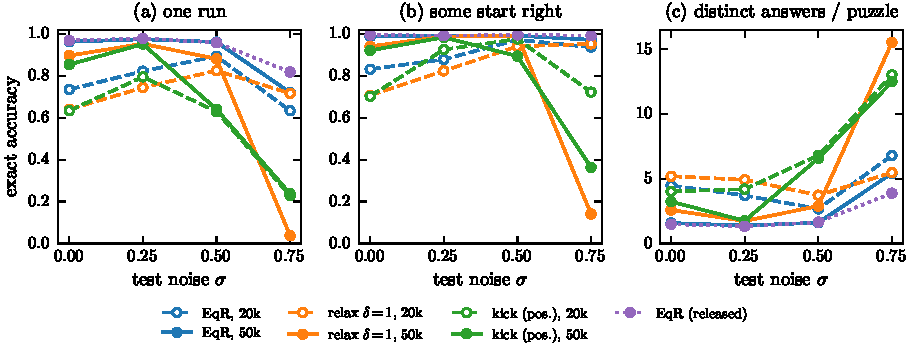
\includegraphics[width=\textwidth]{figures/fig_noise.pdf}
\caption{Multistart against test noise (256 puzzles, 16 starts, depth 256). (a) one run; (b) some start right; (c) distinct answers per
puzzle. Relax at 50k collapses at $\sigma=0.75$ although it tolerated it at 20k.}\label{fig:noise}
\end{figure}

\subsection{Spectra at the end states}\label{sec:spectra}

\begin{table}[t]
\centering\small
\caption{Spectral radius of one outer iteration's Jacobian at noise-free end states (16 right and 16 wrong per arm, power iteration on JVPs), and the share of complex leading Ritz values (Arnoldi, 30 steps).}\label{tab:spectral}
\setlength{\tabcolsep}{4pt}
\begin{tabular}{@{}llrcrr|rr@{}}
\toprule
& & \multicolumn{4}{c|}{right end states} & \multicolumn{2}{c}{wrong end states}\\
arm & steps & $\rho$ & $[q_{10},q_{90}]$ & $\mathbb{C}$ top-1 & $\mathbb{C}$ top-10 & $\rho$ & $\mathbb{C}$ top-1 \\
\midrule
\tabinput{tables/tab_spectral.tex}
\bottomrule
\end{tabular}
\end{table}

\begin{observation}[Right answers attract, wrong end states do not]
In every working model the median spectral radius at right end states is below one and at wrong end states above one
(Table~\ref{tab:spectral}, Figure~\ref{fig:spectral}). Wrong end states after 256 iterations are therefore not stable fixed points but
slow transients or unstable sets, which is why convergence certifies correctness (\S\ref{sec:select}) and why per-instance path independence
separates right from wrong answers \cite{anil2022path}.
\end{observation}

EqR's right answers sit close to criticality and move closer with training ($0.87\to0.93\to0.97$), as reported for converged Sudoku loopers
\cite{labovich2026stability} and in line with the drift of equilibrium models toward critical stability \cite{bai2021jacobian}. The coupled maps contract
much harder ($0.53$--$0.73$). Leading eigenvalues at right answers are complex for EqR and relax at 20k ($88\%$) but real at 50k ($13\%$, $0\%$), and
real for positive kick throughout (Figure~\ref{fig:ritz}): kick is \emph{not} oscillatory at its answers, contrary to a momentum (underdamped)
picture \cite{goh2017momentum}.

One caveat qualifies the comparison. For the coupled maps the spectral radius is almost the same at every right end state
($q_{10}\approx q_{90}$ in Table~\ref{tab:spectral}, e.g.\ $[0.53,0.53]$ for relax at 20k), whereas EqR's varies from puzzle to puzzle. A
puzzle-independent mode of the coupled update, rather than the puzzle's own constraint dynamics, may therefore set the coupled maps' $\rho$;
the leading Ritz values (Figure~\ref{fig:ritz}) are real and tightly clustered, consistent with this. Identifying that mode is left open.

\begin{figure}[t]
\centering
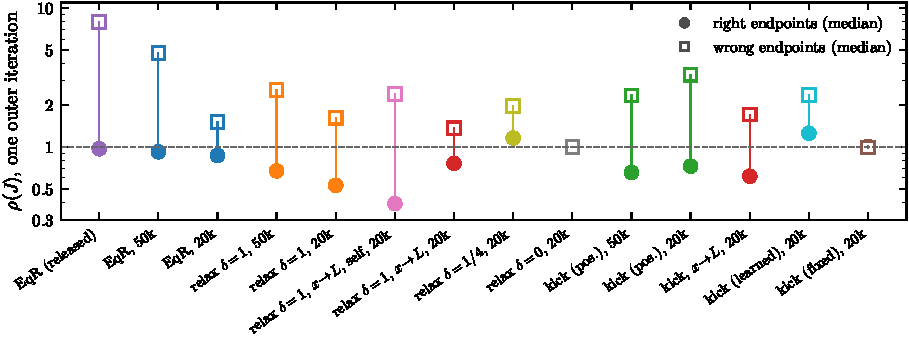
\includegraphics[width=\textwidth]{figures/fig_spectral.pdf}
\caption{Median spectral radius of one outer iteration at right (filled) and wrong (open) end states. Dashed: $\rho=1$.}\label{fig:spectral}
\end{figure}

\begin{figure}[t]
\centering
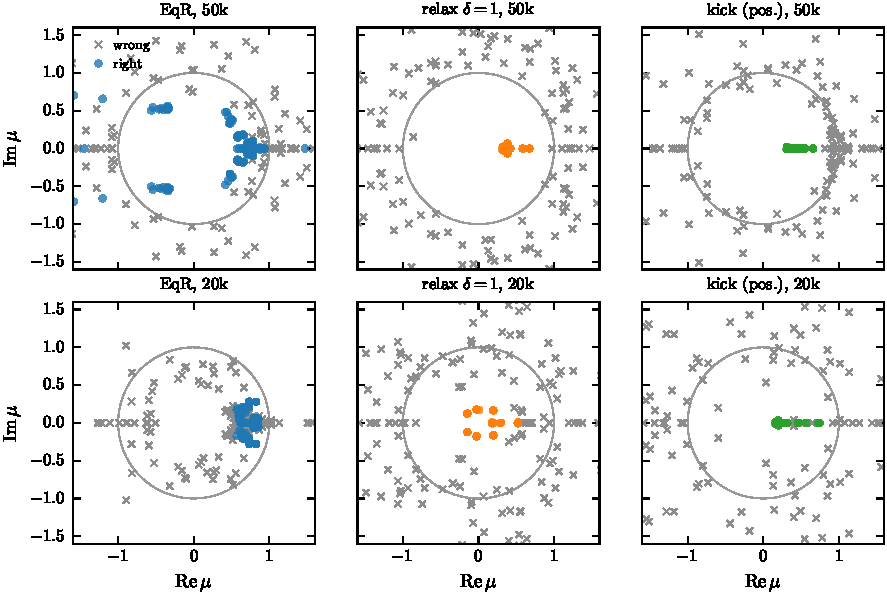
\includegraphics[width=\textwidth]{figures/fig_ritz.pdf}
\caption{Leading Ritz values (top 10 per end state) of one outer iteration's Jacobian. Coloured: right end states; grey crosses: wrong
end states; circle: $|\mu|=1$.}\label{fig:ritz}
\end{figure}

\subsection{Escape under noise}\label{sec:escape}

\begin{table}[t]
\centering\small
\caption{From noise-free end states, $K=32$ iterations at noise $\sigma$: $P(\text{keep}\mid\text{right})\,/\,P(\text{right}\mid\text{wrong})$.}\label{tab:escape}
\begin{tabular}{@{}llccccc@{}}
\toprule
arm & steps & $\sigma=0.1$ & $0.25$ & $0.5$ & $0.75$ & $1.0$\\
\midrule
\tabinput{tables/tab_escape.tex}
\bottomrule
\end{tabular}
\end{table}

Table~\ref{tab:escape} and Figure~\ref{fig:escape}. Up to an arm-specific level $\sigma^\star$ right answers are kept with probability one while
$15$--$33\%$ of wrong end states are rescued; rescue peaks just below $\sigma^\star$. This is the selective destabilisation of spurious attractors
known from Hopfield networks \cite{amit1985storing,coolen2000statics}, and it matches the published observation that noise lowers single-path
quality but raises best-of-$N$ \cite{gladstone2025ebt}. $\sigma^\star$ is above $1$ for EqR at 50k and relax at 20k, between $0.75$ and $1$ for EqR
at 20k, the released EqR and kick at 20k, and between $0.5$ and $0.75$ for relax and kick at 50k. The best test noise for breadth is just below
$\sigma^\star$, so it must be chosen per checkpoint: relax tolerated $\sigma=0.75$ at 20k and collapses there at 50k (single run $3.7\%$),
although its state scale is unchanged; its right answers attract less strongly at 50k ($\rho$ $0.53\to0.68$). Relax $\delta=\frac14$ rescues almost
nothing: its wrong attractors are deep, which is why breadth does not help it.

\begin{figure}[t]
\centering
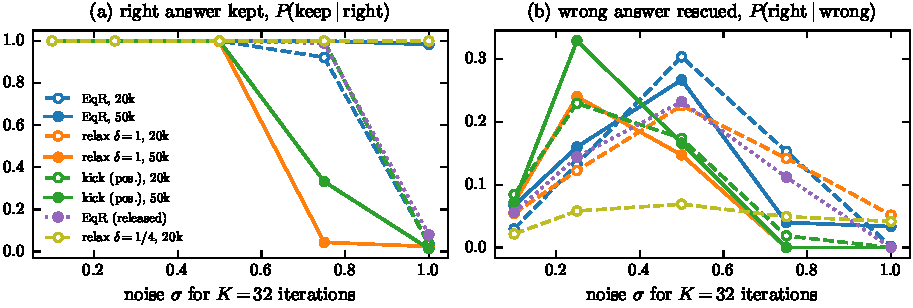
\includegraphics[width=\textwidth]{figures/fig_escape.pdf}
\caption{Escape from noise-free end states after $K=32$ noisy iterations. (a) right answers kept; (b) wrong answers rescued.}\label{fig:escape}
\end{figure}

\begin{figure}[t]
\centering
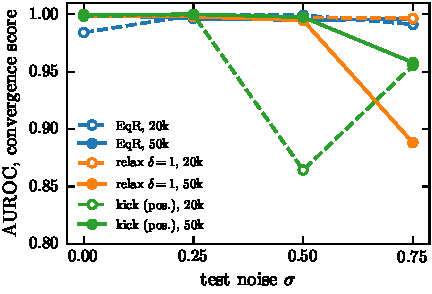
\includegraphics[width=0.55\textwidth]{figures/fig_auroc.pdf}
\caption{AUROC of EqR's convergence score for right vs.\ wrong runs, against test noise.}\label{fig:auroc}
\end{figure}

\subsection{Inside one outer iteration}

\begin{figure}[t]
\centering
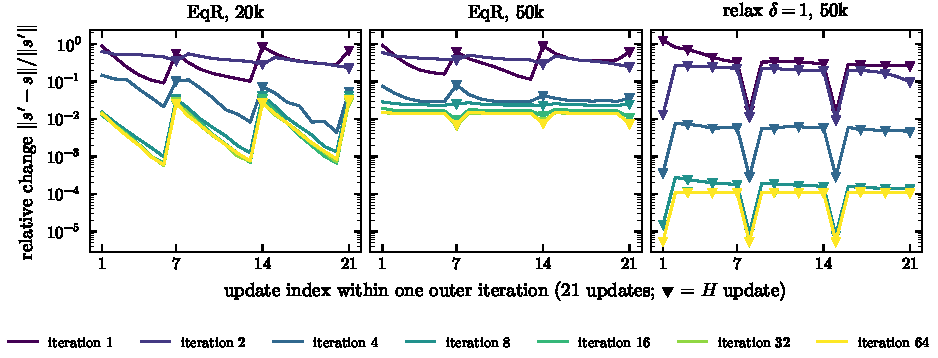
\includegraphics[width=\textwidth]{figures/fig_recursion.pdf}
\caption{Median relative change per update inside one outer iteration (21 updates, $\blacktriangledown$ = $H$ updates), at outer
iterations $1,\dots,64$ from a random start (64 puzzles). EqR at 20k shows hierarchical convergence: $L$ settles within each recursion and
is reset by $H$. At 50k the $L$ changes no longer decay (the 2-cycle of \S\ref{sec:flip}). For relax the dips are the second of two
consecutive $H$ updates at recursion boundaries; the floor near $10^{-4}$ is TF32 round-off on the GPU.}\label{fig:recursion}
\end{figure}

Figure~\ref{fig:recursion}. EqR at 20k shows HRM's \emph{hierarchical convergence} \cite{wang2025hrm}: within each recursion the $L$ change
falls roughly by half per update, then $H$ moves and $L$ restarts. The coupled maps have no such structure (Prop.~\ref{prop:explicit}); every update
changes the state by a similar amount, and the second of two consecutive $H$ updates at each recursion boundary changes almost nothing, so
$2$ of the $21$ evaluations per outer iteration are nearly wasted by the alternating schedule.

\subsection{EqR's inner loop goes through a flip bifurcation}\label{sec:flip}

\begin{figure}[t]
\centering
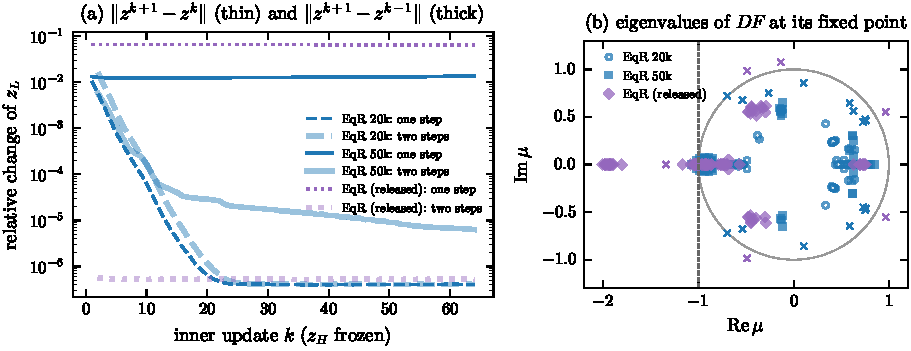
\includegraphics[width=\textwidth]{figures/fig_inner.pdf}
\caption{EqR's inner map $F(\zL)=0.05\zL+0.95\Bk(\zL+\zH+x)$ with $\zH$ frozen at an end state (16 puzzles, local float32).
(a) Median one-step (thin) and two-step (thick) relative change over 64 inner updates: at 20k both vanish (fixed point); at 50k and in the
released model the one-step change stays at $1\%$ and $6\%$ while the two-step change drops to round-off (exact 2-cycle).
(b) Leading eigenvalues of $DF$ at its fixed point (found by damped iteration); crosses: wrong puzzles.}\label{fig:inner}
\end{figure}

\begin{figure}[t]
\centering
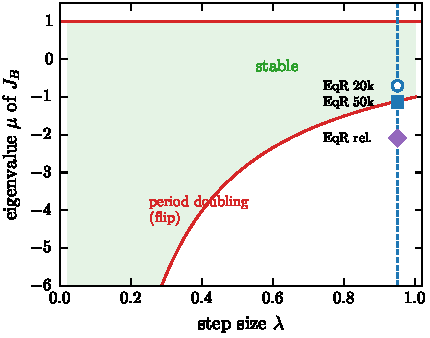
\includegraphics[width=0.5\textwidth]{figures/fig_flip.pdf}
\caption{Stability of $F=(1-\lambda)z+\lambda\tilde\Bk(z)$ along a real eigen-direction $\mu$ of $D\tilde\Bk$ (Prop.~\ref{prop:flip}). Markers:
most negative leading eigenvalue of $DF$ at the inner fixed point (median over right puzzles), mapped to $\mu$ at EqR's $\lambda=0.95$.}\label{fig:flip}
\end{figure}

Figures~\ref{fig:inner} and \ref{fig:flip}. At 20k the inner fixed point is stable (leading eigenvalues of $DF$ near $\pm0.6$ for right
puzzles; wrong puzzles sit at $-1.00$ to $-1.03$). At 50k a cluster of real eigenvalues sits at $-0.93$ to $-1.07$, and in the released checkpoint the
leading eigenvalue is $\approx-1.9$ to $-2.0$, i.e.\ $\mu\approx-2.1$ for the block. The inner fixed point is then unstable and $\zL$ lives on a
stable 2-cycle (two-step Jacobian eigenvalues $0.91$--$0.99$). Because six inner updates are an even number, $\zH$ always reads the same
phase; in the released model $\zH$ is then stationary to $4\times10^{-7}$.

\begin{table}[t]
\centering\small
\caption{Inner-loop length at test time (128 puzzles, one start, 32 outer iterations, local float32): exact accuracy at $\sigma=0$ / $\sigma=0.5$.
Six is the trained value.}\label{tab:lcycles}
\begin{tabular}{@{}lccccc@{}}
\toprule
checkpoint & $L$=4 & 5 & 6 & 7 & 8\\
\midrule
\tabinput{tables/tab_lcycles.tex}
\bottomrule
\end{tabular}
\end{table}

The cycle carries no information the readout uses: odd inner-loop lengths, which make $\zH$ read alternating phases, are as accurate as even
ones (Table~\ref{tab:lcycles}; $\pm2.5$ points at 128 puzzles). We read the period doubling as a by-product of strong negative feedback in the block
combined with EqR's light damping, not as a computational mechanism. By Proposition~\ref{prop:twin} a twin coupling would hold such a cycle as a fixed
point with $L\ne L'$; the twins' merge cosine is therefore a direct readout of whether the twin arms learn the same structure.

%=====================================================================================================
\section{Discussion}

\paragraph{Which properties matter.}
\begin{enumerate}[leftmargin=*,itemsep=1pt]
\item \emph{Attracting right answers and non-attracting wrong ones.} Every working model has it, and it makes selection by convergence or
halting essentially free. Models without it (relax $\delta=0$, $\frac14$; fixed and learned kick) also lose the certificate.
\item \emph{Large, dominant basins for right answers (path independence).} This is where EqR leads, and it grows with training for every arm.
\item \emph{A margin between the noise that breaks wrong attractors and the noise that breaks right ones.} It exists for all working models; its
location $\sigma^\star$ is set by the state scale (exactly predictable, Prop.~\ref{prop:scale}) and by contraction strength, and it moves with training.
\item \emph{Damping of the common mode}, not the volume constraint. The undamped mode of relax is fatal; strong but not maximal damping is best.
\item \emph{An inner equilibrium problem and near-critical contraction} distinguish EqR. The coupled maps contract harder, have an explicit inner
equilibrium, and gain less from training. Whether restoring an implicit inner problem (twin, inner loop) closes the gap is the open question of round three.
\end{enumerate}

\paragraph{Limitations.} All runs use one seed; test-time numbers use 2048 puzzles ($\pm0.5$ points) and the dynamical analysis 256 puzzles
($\pm1$--$2$ points). Spectra use 16 right and 16 wrong end states per arm, and Ritz values from 30 Arnoldi steps approximate only the leading
spectrum. GPU traces ran with TF32 matrix multiplies (round-off $\approx10^{-4}$); the inner-loop analysis was redone locally in float32. The
round-three results are from training curves only.

\paragraph{Next.} Round three at 50k (relax $\delta=2$, twin $\delta=2$, inner loop), with depth$\times$breadth evaluation and the same dynamical
analysis; a per-checkpoint choice of test noise below $\sigma^\star$; a schedule without consecutive $H$ updates; and seeds.

\appendix
\section{Rates, scales and dimensionality}

\begin{table}[h]
\centering\footnotesize
\caption{Rates, the volume bound per outer iteration (Prop.~\ref{prop:volume}), predicted vs.\ measured endpoint RMS of $H$ / $L$
(Prop.~\ref{prop:scale}), and participation ratios $(\sum\ell_i)^2/\sum\ell_i^2$ of the per-token state covariance.}\label{tab:rates}
\setlength{\tabcolsep}{4pt}
\begin{tabular}{@{}llrrrcccc@{}}
\toprule
arm & steps & $\gamma$ & $\alpha$ & $\delta$ & vol.\ bound & RMS pred. & RMS meas. & PR $H$ / $L$\\
\midrule
\tabinput{tables/tab_rates.tex}
\bottomrule
\end{tabular}
\end{table}

\section{Reproduction}
\begin{itemize}[leftmargin=*,itemsep=0pt]
\item Training and evaluation: \nolinkurl{jobs/looped/sudoku_eqr.slurm}, \nolinkurl{jobs/looped/sudoku_scaling.slurm}; summary tables: \nolinkurl{looped/eqr/summarize_sudoku.py}.
\item Dynamical analysis: \nolinkurl{looped/eqr/export_for_analysis.py}, \nolinkurl{looped/eqr/analyze_maps.py} (GPU job \nolinkurl{jobs/looped/sudoku_maps.slurm}), \nolinkurl{looped/eqr/summarize_maps.py}.
\item This note: \nolinkurl{looped/eqr/paper/make_figures.py} and \nolinkurl{make_tables.py}, from the data in \nolinkurl{looped/eqr/paper/data/}.
\end{itemize}

\bibliographystyle{plainnat}
\bibliography{refs}
\end{document}
